\documentclass[a4paper, 12pt]{report}


\usepackage[czech]{babel} % czech language
\usepackage{amssymb} % for math symbols
\usepackage{amsmath} % for math symbols
\usepackage{pdfpages} % for including pdf files
\usepackage{microtype} % better text rendering
\usepackage[T1]{fontenc} % better text rendering
\usepackage{graphicx} % for images
\usepackage[hidelinks]{hyperref} % for clickable links, hidelinks hides the ugly boxes
\usepackage[a4paper,width=160mm,top=25mm,bottom=25mm,bindingoffset=6mm]{geometry} % page layout
\usepackage[pagestyles]{titlesec} % for customizing chapter titles
\usepackage{parskip} % for no indent and space between paragraphs
\usepackage{enumitem} % for customizing lists
\usepackage{fancyhdr} % for customizing headers and footers
\usepackage{bm} % for bold math symbols
\usepackage{tocloft} % for customizing table of contents
\usepackage{multicol} % for multiple columns
\usepackage{hyperref} % for clickable links
\usepackage{textcase} % for uppercasing text
\usepackage{tikz} % for drawing
\usepackage{float} % for floating images
\usepackage{siunitx} % for SI units
\usepackage{caption} % for customizing captions
\usepackage{hhline} % for double lines in tables

% toc font
\renewcommand{\cfttoctitlefont}{\normalfont\Huge\sffamily\bfseries}
\renewcommand{\cftchapfont}{\sffamily\normalsize}
\renewcommand{\cftsecfont}{\sffamily\normalsize}



% for customizing bibliography title
\addto{\captionsczech}{\renewcommand{\bibname}{Seznam zdrojů}}

\fancypagestyle{plain}{
    \renewcommand{\headrulewidth}{0pt}
    \fancyhf{}
    \fancyfoot[C]{\sffamily\selectfont\thepage}
}

\pagestyle{plain}
\fancyhead{}
\fancyhead[R]{\sffamily\rightmark}
\fancyhead[L]{\sffamily\thechapter\ \chaptername}
\setlength{\headheight}{15pt}
\renewcommand{\headrulewidth}{0.4pt}

\renewcommand{\sectionmark}[1]{\markright{#1}}

% for customizing chapter titles
\titleformat{\chapter}[display]{\normalfont\sffamily\bfseries}{}{0pt}{\Huge}

% for customizing section titles
\titleformat{\section}{\normalfont\Large\sffamily\bfseries}{\thesection}{1em}{}

% for customizing subsection titles
\titleformat{\subsection}{\large\sffamily\bfseries}{\thesubsection}{1em}{}

% for customizing subsubsection titles (no new lines after title)
\titleformat{\subsubsection}[runin]{\normalfont\sffamily\bfseries}{\thesubsubsection}{1em}{}

\DeclareCaptionLabelFormat{myformat}{\sffamily#1 #2}
\captionsetup[figure]{labelformat=myformat}



\author{Petr Kotlan}
\title{Optimalizace investičních prostředků z hlediska výnosu fotovoltaických elektráren}
\date{}

\begin{document}

\begin{titlepage}
    \begin{center}
        \Huge

        % \textbf{Univerzita Jana Evangelisty Purkyně \\v Ústí nad Labem}
        \textbf{\textsf{\textls*[-20]{Univerzita Jana Evangelisty Purkyně \\v Ústí nad Labem}}}
            
        \vspace{1cm}
        \LARGE
        \textbf{\textsf{Přírodovědecká fakulta}}
        
        \vspace{2cm}
        \includegraphics[width=0.5\textwidth]{static/PřF-UJEP-logo.png}
        \vspace{3cm}
            
        \textbf{\textsf{Optimalizace investičních prostředků \\z hlediska výnosu fotovoltaických elektráren}}
        
        \vspace{1cm}

        \large
        BAKALÁŘSKÁ PRÁCE

        \vfill

            \begin{flushleft}
                
            \large
            \textbf{Vypracoval:} Petr Kotlan \\
            \vspace{0.3cm}
            \textbf{Vedoucí práce:} Ing. Roman Vaibar, Ph.D., MBA \\
            \vspace{1.5cm}
            \textbf{Studijní program:} Matematika ve firmách a veřejné správě
        \end{flushleft}

        \vspace{1.5cm}
        
        \LARGE
        Ústí nad Labem 2024

    \end{center}
\end{titlepage}

\thispagestyle{empty}
\mbox{}


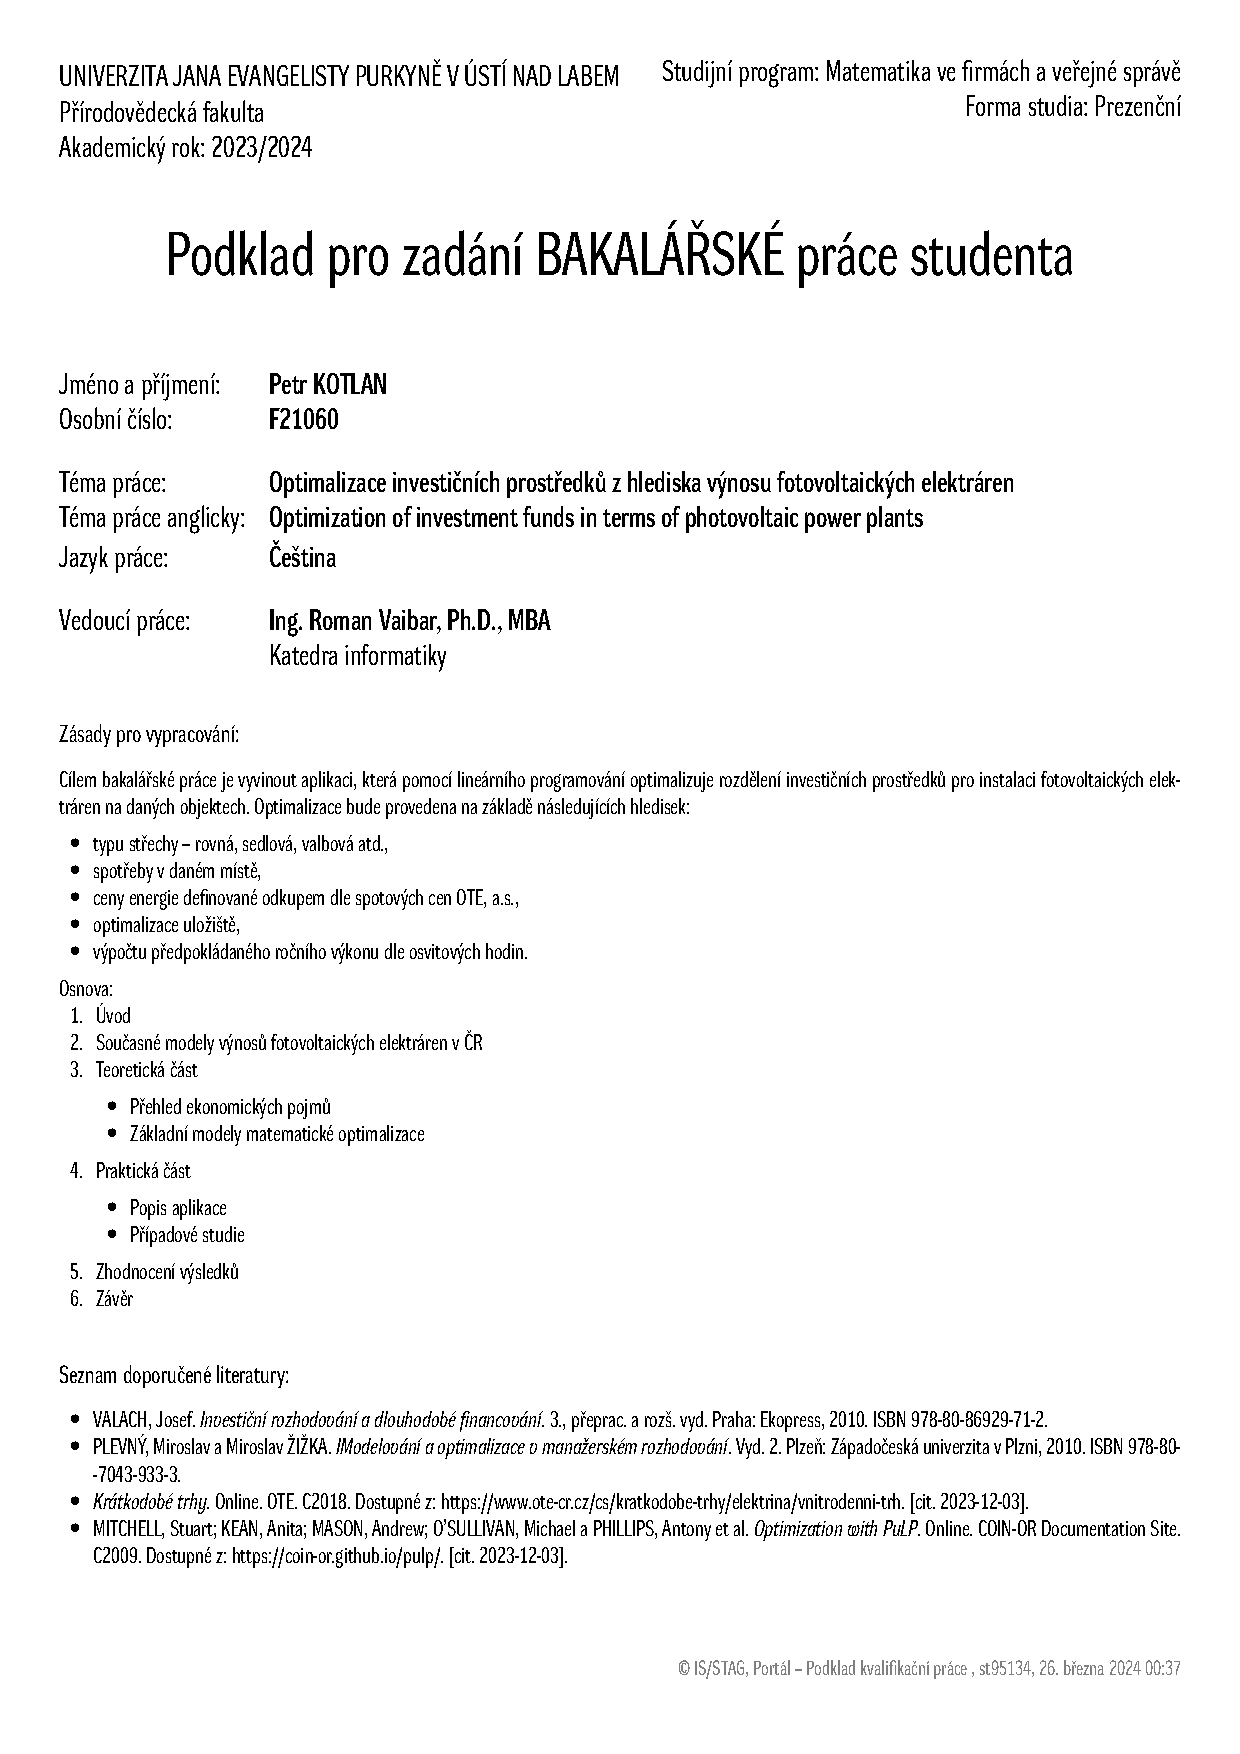
\includepdf[pages=-]{static/podklad_bp.pdf}
\thispagestyle{empty}


\textbf{Prohlášení}

\vspace{1cm}

Prohlašuji, že jsem tuto bakalářskou práci vypracoval samostatně a použil jen pramenů, které
cituji a uvádím v přiloženém seznamu literatury.

\vspace{0.5cm}

Byl jsem seznámen s tím, že se na moji práci vztahují práva a povinnosti vyplývající ze zákona
č. 121/2000 Sb., ve znění zákona č. 81/2005 Sb., autorský zákon, zejména se skutečností,
že Univerzita Jana Evangelisty Purkyně v Ústí nad Labem má právo na uzavření licenční
smlouvy o užití této práce jako školního díla podle § 60 odst. 1 autorského zákona, a s tím, že
pokud dojde k užití této práce mnou nebo bude poskytnuta licence o užití jinému subjektu,
je Univerzita Jana Evangelisty Purkyně v Ústí nad Labem oprávněna ode mne požadovat
přiměřený příspěvek na úhradu nákladů, které na vytvoření díla vynaložila, a to podle
okolností až do jejich skutečné výše.

\vspace{1cm}

\begin{multicols}{2}
    \begin{flushleft}
    V Ústí nad Labem dne \today
    \end{flushleft}

\newcolumn

\begin{flushright}
Podpis: ............................................
\end{flushright}


\end{multicols}

\newpage

\thispagestyle{empty}
\mbox{}
\newpage

\thispagestyle{empty}

% podekovani, vpravo dole
\null
\vfill

\begin{flushright}
    \textit{podekování}
\end{flushright}

\newpage

\thispagestyle{empty}
\mbox{}
\newpage

\thispagestyle{plain}


\textbf{Abstrakt}


\newpage


\thispagestyle{empty}
\mbox{}
\newpage

\tableofcontents

\addcontentsline{toc}{chapter}{Úvod}
\renewcommand{\chaptername}{Úvod}
\chapter*{Úvod}

% \chapter{Současné modely výnosů fotovoltaických elektráren v ČR}
\chapter{Přehled problematiky fotovoltaiky}
\renewcommand{\chaptername}{Přehled problematiky fotovoltaiky}

V úvodní kapitole je popsána základní problematika fotovoltaických elektráren.
Je zde uveden základní technický popis, jednotlivé komponenty ze kterých se elektrárna skládá a druhy systémů, které se v praxi využívají.

\section{Technický popis fotovoltaických elektráren}

% https://www.fotovia.cz/komponenty-fve
% TODO: vysvetlit proc to tu je

% schema tvary

\subsection{Veličiny}

\subsubsection{Watt} je jednotkou výkonu a rovná se vykonané práci za jendotku času.
Značíme ji symbolem \si{\watt}.

\subsubsection{Watt hodina} je jednotkou energie a rovná se práci stroje o výkonu jednoho wattu, který pracuje po dobu jedné hodiny.
Značíme ji symbolem \si{\watt\hour}. Při měření spotřeby elektřiny se nejčastěji se užívá v násobku kilowatt hodiny (\si{\kWh}).

\subsubsection{Killowatt--peak} je jednotkou špičkového výkonu fotovoltaické elektrárny. Tento výkon je při standardních testovacích podmínkách.


\subsection{Komponenty fotovoltaické elektrárny}
To, jaké komponenty se investor rozhodne koupit do svého fotovoltaického systému, může zásadně ovlivnit návratnost této investice.
Některé komponenty jsou pro elektrárnu nezbytné, jiné slouží k optimalizaci výkonu při různých podmínkách či specifickém využití.
Zde uvádím některé základní komponenty fotovoltaické elektrárny.

\subsubsection{Fotovoltaické panely}

jsou nezbytnou součástí každé fotovoltaické elektrárny.
Jejich hlavním úkolem je absorbovat sluneční záření a přeměnit ho na elektrickou energii.

\subsubsection{Baterie}

(nebo také akumulátory) slouží k ukládání přebytků energie, které nebyly spotřebovány.
Dělíme je na virtuální uložiště a fyzické uložiště.

\begin{itemize}
    \item \textbf{Virtuální uložiště} -- funguje na základě podepsání smlouvy s distributorem. Přebytky vyrobené energie se posílají do veřejné sítě, odkud se v případě potřeby mohou odčerpat.  Ve virtuální baterii můžete uložit tolik energie, kolik vám smluvně umožňuje distributor. Mají několik nevýhod:
    \begin{itemize}
        \item je to komerční produkt, který nenabízí všichni distributoři a nikde se negarantují stálé podmínky,
        \item platíte za využívání paušální poplatek,
        \item v případě výpadku elektřiny nemáte záložní zdroj energie.
    \end{itemize}
    \item \textbf{Fyzické bateriové uložiště} -- je zařízení, které je uložené v domě. Vyrobená energie se do baterií ukládá a v případě potřeby se z nich odebírá. Nevýhodou fyzické baterie je její kapacita.
\end{itemize}


% \subsubsection{Virtuální uložiště}
% funguje na základě podepsání smlouvy s distributorem. Přebytky vyrobené energie se posílají do veřejné sítě, odkud se v případě potřeby mohou odčerpat.
% Virtuální úložiště nejsou plnou náhradou fyzických baterií. Mají několik nevýhod:

% \begin{itemize}
%     \item je to komerční produkt, který nenabízí všichni distributoři a nikde se negarantují stálé podmínky,
%     \item platíte za využívání paušální poplatek,
%     \item v případě výpadku elektřiny nemáte záložní zdroj energie. 
% \end{itemize}

% \subsubsection{Fyzické bateriové uložiště} je zařízení, které je uložené v domě. Vyrobená energie se do baterií ukládá a v případě potřeby se z nich odebírá.
% Nevýhodou fyzické baterie je její kapacita. Ve virtuální baterii můžete uložit tolik energie, kolik vám smluvně umožňuje distributor.


\subsubsection{Invertor}

(nebo také měnič či střídač) je podobně jako fotovoltaické panely
nezbytnou součástí každé fotovoltaické elektrárny.
Jeho hlavní funkcí je přeměna stejnosměrného proudu na proud střídavý.
Inverotr rozděluje vyrobenou energii do tří fází. To kolik dávkuje do jednotlivých fází záleží na typu invertoru.

\begin{itemize}
    \item Symetrikcý invertor -- levnější typ, dávkuje elektřinu rovnoměrně do všech tří fází.
    \item Asymetrický invertor -- dražší typ, při dávkování zohledňuje spotřebu na všech fázích.
\end{itemize}

Pokud by tedy například fotovoltaika vyrobila 6 \si{\kWh} elektřiny a spotřeba by na jednotlivých fázích vypdala následovně:

\begin{itemize}
    \item Fáze 1: 3 \si{\kWh}
    \item Fáze 2: 2 \si{\kWh}
    \item Fáze 3: 0.5 \si{\kWh}
\end{itemize}

Symetrický invertor rozdělí elektřinu rovnoměrně (2 \si{\kWh} na každou fázi), takže na fázi 2 a 3 vznikne přebytek, který se pošle do sítě a na fázi 1 energie chybí, tzn. musí se dobrat ze sítě.
Asymetrický invertor elektřinu rozdělí tak, že nebude nutné ze sítě nic dobírat, ani do ní nic posílat.  

\subsubsection{Optimizér}
je zařízení, které se připojuje k jednotlivým fotovoltaickým panelům. Výkon elektrárny se odvíjí od výkony nejméně vákoného článku.
V případě že je snížen výkon jednoho panelu, optimizér zajistí přemostění tohoto panelu.


\subsection{Druhy fotovoltaických systémů}
% https://www.fotovia.cz/blog/typy-fotovoltaickych-elektraren

Rozdílem mezi jednotlivými druhy fotovoltaických systémů je jejich napojení do veřejné elektrické sítě a integrace akumulátorů.
Podle těchto kritérií je lze rozdělit do tří základních kategorií:

\begin{itemize}
    \item ostrovní
    \item standardní
    \item hybridní
\end{itemize}

\subsubsection{Ostrovní elektrárna}

(tzv. off-grid) je samostatný systém, který není připojen k elektrické síti.
Klíčovou částí toho systému je baterie (akumulátor), která slouží k ukládání přebytků energie.
Jsou užitečné v oblastech, kde připojení k elektrické síti není možné.

\begin{multicols}{2}
    \textbf{Výhody:}
    \begin{itemize}[leftmargin=*]
        \item nezávislost na dodavatelích elektřiny,
        \item pokud dojde k výpadku elektřiny, ostrovní elektrárna bude sloužit jako záložní zdroj,
    \end{itemize}
    
    \columnbreak
    
    \textbf{Nevýhody:}
    \begin{itemize}[leftmargin=*]
        \item počáteční náklady mohou být vyšší, kvůli potřebě akumulátorů,
        \item baterie vyžadují pravidelnou údržbu.
    \end{itemize}
\end{multicols}

\begin{figure}[h]
    \centering
    \begin{tikzpicture}[>=stealth,thick]
        % Nodes
        \node[draw, minimum height=1cm] (panel) at (0,0) {Panel};
        \node[draw, circle] (inverter) at (3,0) {Invertor};
        \node[draw] (baterie) at (3,-2) {Baterie};
        \node[draw, circle] (odb) at (6,0) {Spotřebič};
        % Arrows
        \draw[->] (panel) -- (inverter);
        \draw[->] (inverter) -- (baterie);
        \draw[->] (baterie) -- (inverter);
        \draw[->] (inverter) -- (odb);

    \end{tikzpicture}
    \caption{Schéma off-grid fotovoltaické elektrárny}
    \label{fig:offgrid_schema}
\end{figure}

\subsubsection{Standardní elektrárna}

Standardní (tzv. on-grid) fotovoltaická elektrárna je připojena k elektrické síti.
Veškerou přebytečnou energii lze prodat dodavateli elektřiny.

\begin{multicols}{2}
    \textbf{Výhody:}
    \begin{itemize}[leftmargin=*]
        \item možnost prodeje přebytků elektřiny,
        \item dlouhá životnost, malá potřeba údržby.
    \end{itemize}
    
    \columnbreak
    
    \textbf{Nevýhody:}
    \begin{itemize}[leftmargin=*]
        \item závislost na síti,
        \item závislost na slunečním záření.
    \end{itemize}
\end{multicols}


\begin{figure}[H]
    \centering
    \begin{tikzpicture}[>=stealth,thick]
        % Nodes
        \node[draw, minimum height=1cm] (panel) at (0,0) {Panel};
        \node[draw, circle] (inverter) at (3,0) {Invertor};
        \node[draw, circle] (odb) at (6,0) {Spotřebič};
        \node[draw, minimum width=2cm] (sita) at (3,-2) {Elektrická síť};
        % Arrows
        \draw[->] (panel) -- (inverter);
        \draw[->] (inverter) -- (odb);
        \draw[->] (inverter) -- (sita);

    \end{tikzpicture}
    \caption{Schéma on-grid fotovoltaické elektrárny}
    \label{fig:ongrid_schema}
    \end{figure}


\subsubsection{Hybridní elektrárna}

kombinuje výhody ostrovních a standardních systémů.
Jsou připojeny k elektrické síti, ale zároveň mají akumulátory, které slouží jako záložní zdroj energie.

\begin{multicols}{2}
    \textbf{Výhody:}
    \begin{itemize}[leftmargin=*]
        \item uložení přebytků energie,
        \item větší energetická nezávislost.
    \end{itemize}
    
    \columnbreak
    
    \textbf{Nevýhody:}
    \begin{itemize}[leftmargin=*]
        \item vysoké počáteční náklady,
        \item baterie vyžadují pravidelnou údržbu.
    \end{itemize}

\end{multicols}

\begin{figure}[h]
    \centering
    \begin{tikzpicture}[>=stealth,thick]
        % Nodes
        \node[draw, minimum height=1cm] (panel) at (0,0) {Panel};
        \node[draw, circle] (inverter) at (3,0) {Invertor};
        \node[draw] (baterie) at (2,-2) {Baterie};
        \node[draw, circle] (odb) at (6,0) {Spotřebič};
        \node[draw, minimum width=2cm] (sita) at (4.5,-2) {Elektrická síť};
        % Arrows
        \draw[->] (panel) -- (inverter);
        \draw[->] (inverter) -- (baterie);
        \draw[->] (baterie) -- (inverter);
        \draw[->] (inverter) -- (odb);
        \draw[->] (inverter) -- (sita);

    \end{tikzpicture}
    \caption{Schéma hybridní fotovoltaické elektrárny}
    \label{fig:hybrid_schema}
\end{figure}


\section{Jak fotovoltaika šetří peníze}
% https://oze.tzb-info.cz/fotovoltaika/24229-stroj-na-penize-fotovoltaika-pri-vysokych-cenach-elektriny-usetri-desetitisice-korun-rocne

\chapter{Investiční možnosti}
\renewcommand{\chaptername}{Investiční možnosti}

\chapter{Teoretická část}
\renewcommand{\chaptername}{Teoretická část}

Tato kapitola je rozdělena do dvou částí. První část se zabývá základními ekonomickými pojmy využívanými v investiční analýze.
Druhá část se zabývá matematickou optimalizací metodou lineárního programování.

Tato část se nejprve zabývá pojmy a ukazateli z oblasti investic.
Poté jsou popsány metody a základní modely lineárního programování.

\section{Investice}

% TODO: citace

Investicí se označuje takové vynaložení finančních prostředků, které se v budoucnu nějakou mírou zhodnotí.
Investice se dělí na reálné a finanční. Mezi reálné patří například investice do nemovitostí, drahých kovů nebo uměleckých děl, tedy do hmotného majetku.
Finanční investice jsou investice do finančních aktiv, jako jsou akcie nebo dluhopisy.
Jako základní pomůcka k posouzení investic slouží \textit{investiční trojúhelník}, který zahrnuje tři základní parametry investice: rizikovost, výnosnost a likviditu.
Obecně platí, že s rostoucím výnosem roste rizikovost a klesá likvidita a naopak.

\subsection{Investiční možnosti}

Záměrem je porovnat investici do fotovoltaické elektrárny s jinými možnostmi.
% vysvetlit proc bereme pouze financi investice


\subsubsection{Spořící účty}
mají zpravidla vyšší úrokovou sazbu než běžné účty.
Výhodou je vysoká likvidita.
V současnosti se úroková sazba pohybuje okolo 4.5\% p.a.

\subsubsection{Dluhopisy} jsou cenné papíry,
které držiteli garantuje pravidelný výnos a jeho následný zpětný odkup.
Známým druhem dluhopisů jsou státní dluhopisy, které Ministerstvo financí prodává několika největším bankám a obchodníkům.
Ti je pak prodávají dalším zájemcům.


\subsubsection{Akcie} je cenný papír, který představuje podíl na kapitálu akciové společnosti.
Majitel akcií má právo na tzv. \textit{dividenda}, tedy podíl na zisku společnosti.


\subsection{Ukazatele výnosnosti investice}

Ukazatele výnosnosti investic jsou klíčovými nástroji při hodnocení investičních rozhodnutí
Poskytují investorům přehled o efektivitě investice a umožňují vzájemné porovnání různých investičních příležitostí.



\subsubsection{Výnosnost investice}
($ROI$ -- Return of Investment)
% https://www.moneta.cz/slovnik-pojmu/detail/roi
vyjadřuje zisk nebo ztrátu z investice v procentech.

\begin{equation}
    ROI = \frac{(P_1 + P_2 + \ldots + P_t) - K}{K} \cdot 100,
\end{equation}

kde
\begin{itemize}[label={}]
    \item $t$ -- počet let,
    \item $P_1, P_2, \ldots, P_t$ -- peněžní příjmy z investice v jednotlivých letech,
    \item $K$ -- kapitálový výdaj,
    \item $ROI$ -- návratnost investice.
\end{itemize}

\subsubsection{Diskontované cash-flow}
($DCF$ -- Discounted Cash Flow)
vyjadřuje současnou hodnotu budoucích peněžních toků.

\begin{equation}
    DCF = \frac{P_1}{(1+i)} + \frac{P_2}{(1+i)^2} + \ldots + \frac{P_t}{(1+i)^t},
\end{equation}

kde
\begin{itemize}[label={}]
    \item $t$ -- počet let,
    \item $P_1, P_2, \ldots, P_t$ -- peněžní příjmy z investice v jednotlivých letech,
    \item $i$ -- úroková míra (diskontní sazba),
    \item $DCF$ -- diskontované cash-flow.
\end{itemize}

\subsubsection*{Čistá současná hodnota}
($NPV$ -- Net Present Value)
vyjadřuje současnou hodnotu budoucích peněžních toků po odečtení kapitálového výdaje.

\begin{equation}    
NPV = \frac{P_1}{(1+i)} + \frac{P_2}{(1+i)^2} + \ldots + \frac{P_t}{(1+i)^t} - K,
\end{equation}

kde
\begin{itemize}[label={}]
    \item $t$ -- počet let,
    \item $P_1, P_2, \ldots, P_t$ -- peněžní příjmy z investice v jednotlivých letech,
    \item $K$ -- kapitálový výdaj,
    \item $i$ -- úroková míra (diskontní sazba),
    \item $NPV$ -- čistá současná hodnota.
\end{itemize}

\subsubsection*{Vnitřní výnosové procento}
($IRR$ -- Internal Rate of Return)
je úroková míra, při níž se současná hodnota peněžních příjmů z investice rovná kapitálovým výdajům. Investice se považuje za výhodnou, když $IRR$ představuje vyšší úrok, než je požadovaná minimální výnosnost investice.

\begin{equation}
    \frac{P_1}{(1+IRR)} + \frac{P_2}{(1+IRR)^2} + \ldots + \frac{P_t}{(1+IRR)^t} = K,
\end{equation}

kde
\begin{itemize}[label={}]
    \item $t$ -- počet let,
    \item $P_1, P_2, \ldots, P_t$ -- peněžní příjmy z investice v jednotlivých letech,
    \item $K$ -- kapitálový výdaj,
    \item $IRR$ -- vnitřní výnosové procento.
\end{itemize}


% \section{Základní modely matematické optimalizace}
\subsection{Formulace úlohy lineárního programování}

\subsubsection{Účelová funkce}


Účelová funkce je lineární funkcí $n$ proměnných ve tvaru

\begin{equation}
    z = c_1x_1 + c_2x_2 + \ldots + c_nx_n ,
\end{equation}


kde $c_1, c_2, \ldots c_n$ jsou konstanty, které nazýváme \textit{cenové koeficienty} nebo \textit{koeficienty účelové funkce} a 
$x_1, x_2, \ldots x_n$ jsou \textit{strukturní neznámé}.

Účelová funkce se buď maximalizuje
% TODO: equation, labely
% $$ \max z = c_1x_1 + c_2x_2 + \ldots + c_nx_n ,$$
\begin{equation}
    \max z = c_1x_1 + c_2x_2 + \ldots + c_nx_n ,
\end{equation}

nebo minimalizuje

% $$ \min z = c_1x_1 + c_2x_2 + \ldots + c_nx_n .$$
\begin{equation}
    \min z = c_1x_1 + c_2x_2 + \ldots + c_nx_n .
\end{equation}

\subsubsection{Omezující podmínky}

Omezující podmínky jsou lineární rovnice nebo nerovnice ve tvaru


$$ a_{11}x_1 + a_{12}x_2 + \ldots + a_{1n}x_n \ \lesseqgtr \ b_1 ,$$
$$ a_{21}x_1 + a_{22}x_2 + \ldots + a_{2n}x_n \ \lesseqgtr \ b_2 ,$$
$$ \vdots $$
$$ a_{m1}x_1 + a_{m2}x_2 + \ldots + a_{mn}x_n \ \lesseqgtr \ b_m ,$$
% TODO: doslovne prepisy

nebo

$$ a_{11}x_1 + a_{12}x_2 + \ldots + a_{1n}x_n \geq b_1 ,$$
$$ a_{21}x_1 + a_{22}x_2 + \ldots + a_{2n}x_n \geq b_2 ,$$
$$ \vdots $$
$$ a_{m1}x_1 + a_{m2}x_2 + \ldots + a_{mn}x_n \geq b_m ,$$

kde $a_{ij}$ jsou konstanty, které nazýváme \textit{strukturní koeficienty} nebo \textit{koeficienty omezení}, $b_i$ jsou konstanty (tzv. \textit{požadavková čísla})
a $x_1, x_2, \ldots x_n$ jsou \textit{strukturní neznámé}.

Zároveň omezující podmínky vymezují pro každou proměnnou $x_1, x_2, \ldots x_n$ množinu hodnot, kterýh může nabývat. 
Nejčastěji se jedná o podmínky tvaru $x_i \geq 0$ (nezápornost).
Jinými případy mohou být například podmínky tvaru $x_i \leq 0$ (nekladnost) nebo $x_i$ může nabývat libovolné hodnoty („neomezeno“).

\subsection{Maticové vyjádření}

Můžeme vyjádřit účelovou funkci jako $$ z = \bm{c}^T\bm{x} ,$$
kde $\bm{c} = (c_1, c_2, \ldots, c_n)^T$ je vektor cenových koeficientů a $\bm{x} = (x_1, x_2, \ldots, x_n)^T$ je vektor strukturních neznámých.

Omezující podmínky můžeme vyjádřit jako maticový součin

$$ \bm{A}\bm{x} \leq \bm{b} ,$$

kde $\bm{A}$ je matice strukturních koeficientů a $\bm{b}$ je vektor pravých stran omezujících podmínek.

\subsection{Typy úloh lineárního programování}

\chapter{Praktická část}
\renewcommand{\chaptername}{Praktická část}

\section{Popis aplikace}
\subsection{Data}

\subsubsection*{Český hydrometeorologický ústav}

\textbf{ČHMÚ}

\href{https://www.chmi.cz/files/portal/docs/meteo/ok/open_data_2023/Podminky_uziti_udaju.pdf}{Podmínky užití dat}

\subsubsection*{OTE, a.s.}

OTE (Otevřený trh s elektřinou)



\section{Případové studie}

\renewcommand{\chaptername}{Zhodnocení výsledků a závěr}
\chapter{Zhodnocení výsledků a závěr}

\addcontentsline{toc}{chapter}{Seznam zdrojů}
\bibliographystyle{plain}
\begin{thebibliography}{9}
    \bibitem{demel}
    DEMEL, Jiří. \textit{Operační výzkum}. Dostupné z: \url{https://kix.fsv.cvut.cz/~demel/ped/ov/ov.pdf}.
    
    \bibitem{fotovia-komponenty}
    \textit{Komponenty FVE}. Online. Fotovia. 2023. Dostupné také z: \url{https://www.fotovia.cz/komponenty-fve}.
    
    \bibitem{fotovia-typy}
    \textit{Typy fotovoltaických elektráren}. Online. Fotovia. 2023. Dostupné také z: \url{https://www.fotovia.cz/blog/typy-fotovoltaickych-elektraren}.
    
    \bibitem{ote}
    \textit{Krátkodobé trhy}. Online. OTE. C2018. Dostupné z: \url{https://www.ote-cr.cz/cs/kratkodobe-trhy/elektrina/vnitrodenni-trh}.
    
    \bibitem{tzb-jakfotovoltaikasetripenize}
    \textit{Stroj na peníze: Fotovoltaika při vysokých cenách elektřiny ušetří desetitisíce korun ročně}. Online. TZB-info - Portál pro stavebnictví, technická zařízení budov. 2001. Dostupné z: \url{https://oze.tzb-info.cz/fotovoltaika/24229-stroj-na-penize-fotovoltaika-pri-vysokych-cenach-elektriny-usetri-desetitisice-korun-rocne}.

    \bibitem{tzb-info}
    \textit{Fotovoltaika}. Online. TZB-info - Portál pro stavebnictví, technická zařízení budov. 2001.. Dostupné z: \url{https://oze.tzb-info.cz/fotovoltaika}.

    \bibitem{matematika_pro_ekonomy}
    STOLÍN, Radek. \textit{Matematika pro ekonomy}. 2., upr. vyd. Jihlava: Vysoká škola polytechnická Jihlava, 2011. ISBN ISBN978-80-87035-35-1.

    \bibitem{python-pulp}
    MITCHELL, Stuart; KEAN, Anita; MASON, Andrew; O'SULLIVAN, Michael a PHILLIPS, Antony. \textit{Optimization with PuLP}. Online. COIN-OR Documentation Site. C2009. Dostupné z: \url{https://coin-or.github.io/pulp/}.
    
    \bibitem{moneta}
    \textit{Slovník pojmů z finančnictví a bankovnictví}. Online. MONETA Money Bank. Dostupné z: https://www.moneta.cz/slovnik-pojmu.

    \bibitem{chmu}
    \textit{ČHMÚ}. Online. Dostupné z: \url{https://www.chmi.cz/}.

\end{thebibliography}

\end{document}